\section{Learning to Rank}
\begin{itemize}
	\item Main issue in information retrieval is to determine whether document $d$ is relevant for query $q$
	\item Common relevance signals include TF-IDF, BM25, document popularity etc.
	\item But: what signals to use/how to combine these signals? There is not a single relevance signal "to rule them all" $\implies$ combine all signals in a model
	\item Simplest combination method: linear model $f(\bm{d},\bm{\theta}) = \sum\limits_{i=1}^{|d|} \theta_i d_i$ where $\bm{d}$ represents the different signals for document-query pair
	\item Task: find the optimal parameter set $\bm{\theta}$, commonly by Machine Learning techniques (linear regression)
\end{itemize}
\subsection{Offline Learning To Rank}
\begin{itemize}
	\item Given an annotated dataset of relation document and relevance/ranking
	\item There are three different approaches
	\begin{enumerate}
		\item \textbf{Pointwise}: optimize models $f(\bm{d},\bm{\theta})$ to predict relevancy of a document. This can be recasted in a regression problem with loss:
		$$\mathcal{L}=\sum_{\bm{d}} \left(f(\bm{d},\bm{\theta}) - \text{relevancy}(d,q)\right)^2$$
		However, this approach does not consider the application of ranking where only the final order is important, but not the single scores.
		\item \textbf{Pairwise}: optimize regarding the total order of the documents and not specific relevance scores. The loss can be expressed by:
		$$\mathcal{L}=\sum_{d\succ d'}\left[f(\bm{d'},\bm{\theta}) - f(\bm{d},\bm{\theta})\right]$$ 
		where $d\succ d'$ means that $d'$ is the successor of $d$ in the labeled ranking. Nevertheless, this method does not take into account that only a subpart (top 10) of the collection is actually presented to the user.
		\item \textbf{Listwise}: optimize regarding ranking metrics like $DCG$. Thus, the loss could be:
		$$\mathcal{L} = -nDCG(f(\cdot,\bm{\theta}))$$
		The problem is that most ranking metrics are not differentiable. There are heuristic approaches to still optimize with respect to such metrics. 
	\end{enumerate}
	\item Problems with offline Learning to Rank: similar to offline evaluation in Section~\ref{sec:offline_eval_problems}
	\begin{itemize}
		\item All described methods require an annotated dataset which contains either relevance labels for each document-query pair or a ranking over the whole collection.
		\item Creating such is time consuming and expensive
		\item Impossible to personalize for a user (everyone prefers a little bit different documents). Also, annotators and users might disagree in some points $\implies$ dataset does not fully reflect user behavior
		\item Can change over time
	\end{itemize}
\end{itemize}
\subsection{Online Learning to Rank}
\begin{itemize}
	\item Learn from implicit user feedback
	\begin{itemize}
		\item Might be noisy
		\item Consider position bias (higher rank is more frequently clicked) and selection bias (only a limited set of documents is presented to the user)
	\end{itemize}
	\item Online Learning to Rank methods can learn from user interactions, \textbf{and} control the results which are displayed/presented to the user
	\item Thus, these methods can be more efficients as they control over what data is actually gathered
	\item A general online learning to rank technique is visualized in Figure~\ref{img:learning_to_rank_online_overview}
	\begin{figure}[ht]
		\centering
		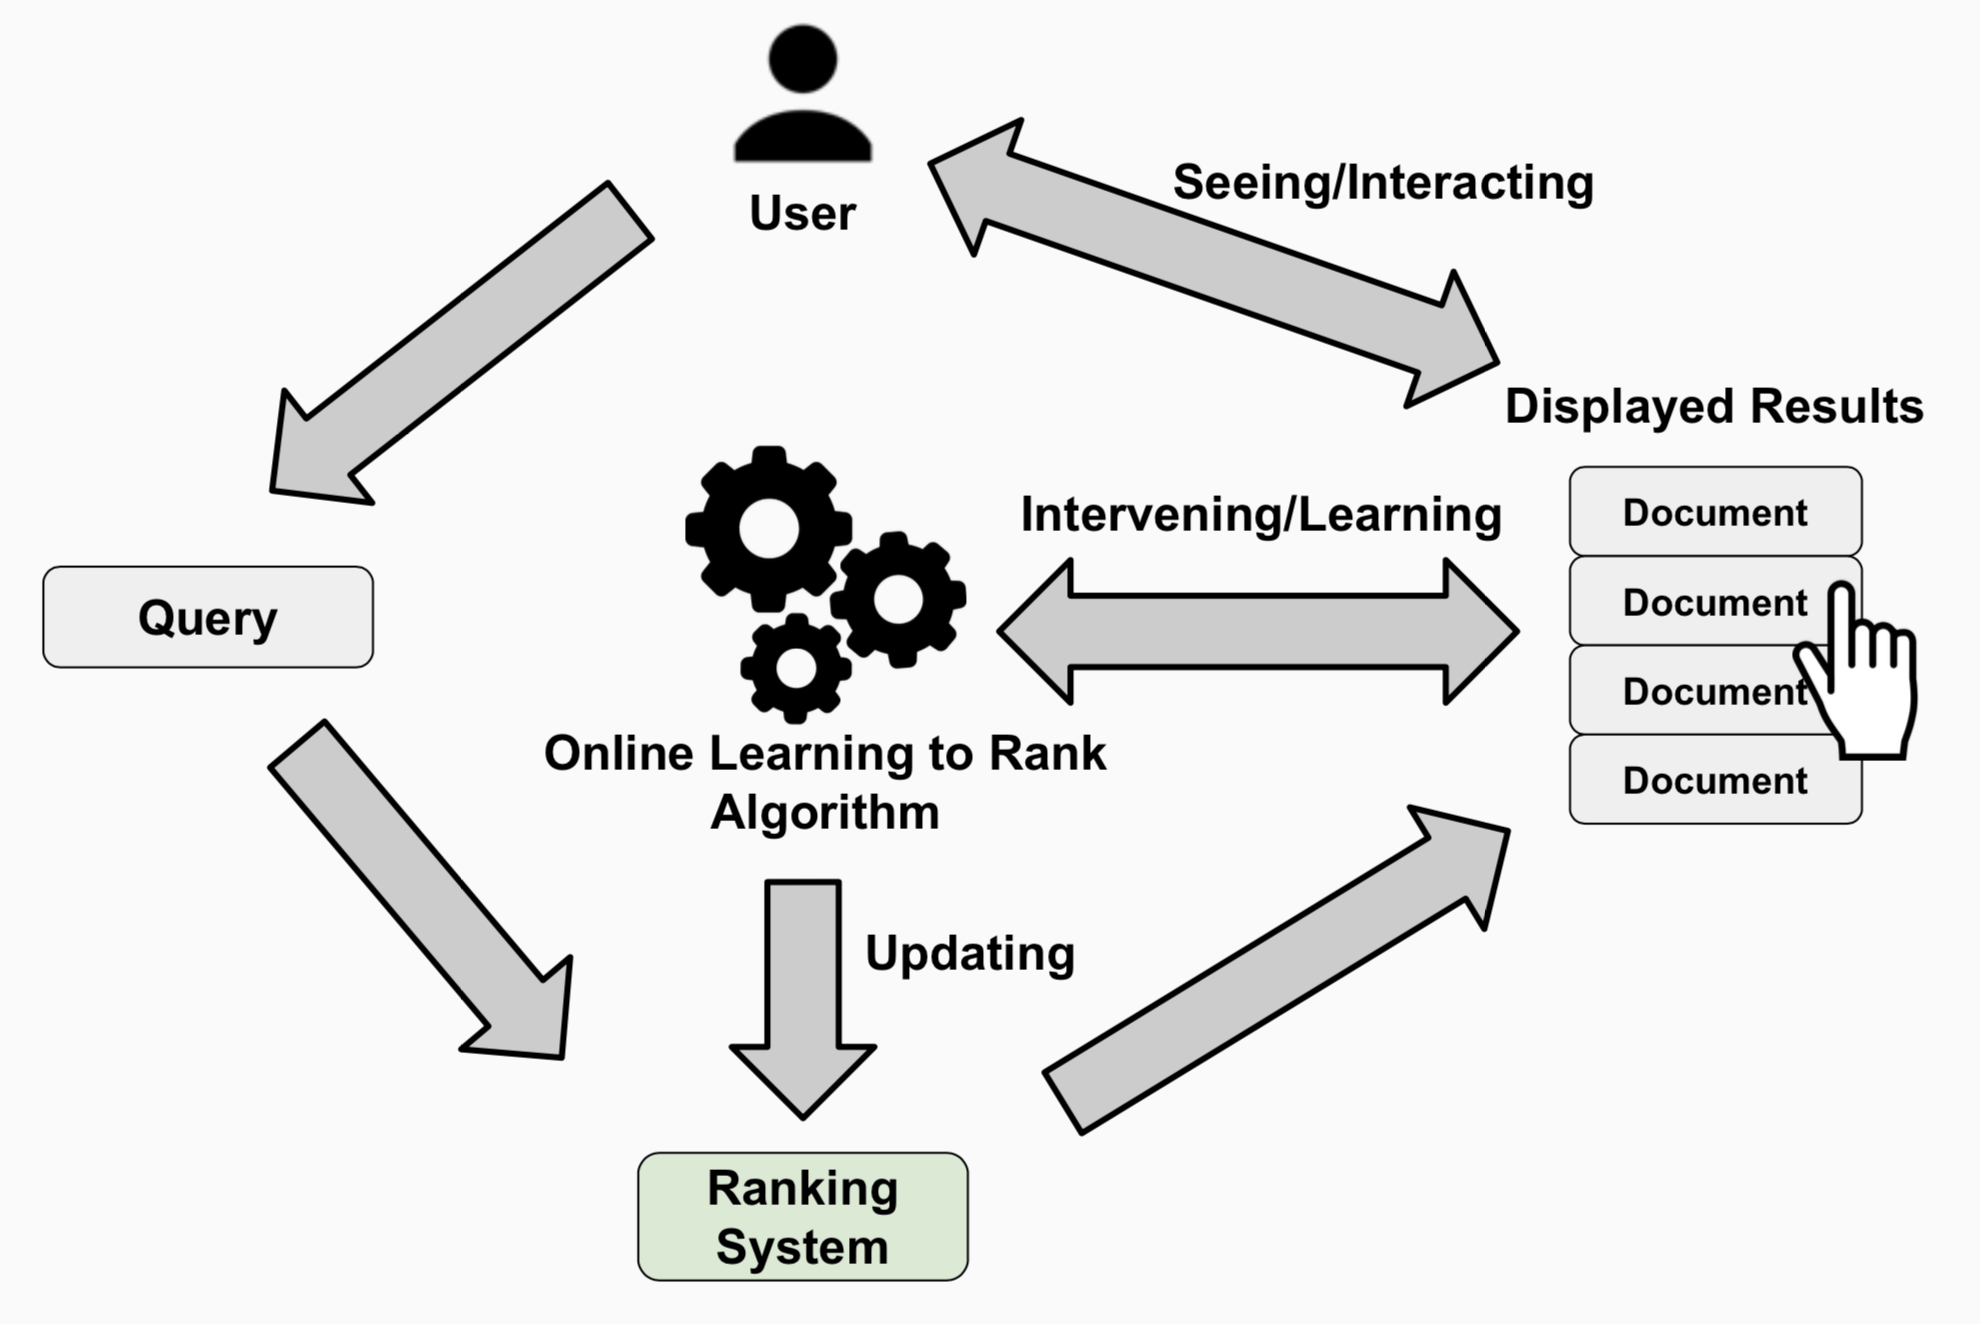
\includegraphics[width=0.4\textwidth]{figures/learning_to_rank_online_overview.png}
		\caption{Overview of the general concept of online learning to rank}
		\label{img:learning_to_rank_online_overview}
	\end{figure}
	\begin{itemize}
		\item The user enters a query, for which the ranking algorithm generates a list of documents
		\item The Online Learning to Rank system interacts with the results by adding and/or removing documents from the ranking. This can also include interleaving with another, slightly changed ranking algorithm
		\item User interacts with the displayed result and gives implicit feedback.
		\item The Online Learning to Rank algorithm updates the ranking parameters according to the analyzed feedback
	\end{itemize}
	\item \textbf{Advantages}: learns directly from the user, is more responsive by immediately adapting its parameters
	\item \textbf{Risks}:
	\begin{itemize}
		\item Unreliable methods will affect/worsen user experiences immediately.
		\item (Noisy) clicks can easily bias or even manipulate search engines
		\item \textbf{Self-confirming loop}
		\begin{itemize}
			\item If an irrelevant document was clicked by random, the system still perceives that this document is relevant and will change its parameters accordingly
			\item Thus, the random document will be placed higher in future ranks. However, also similar documents to the irrelevant one will have an increased relevance score and will probably occur at a high position
			\item Most likely, the next clicked document will be one of the highest ones which were irrelevant $\implies$ entering a self-confirming loop
			\item Due to bias and noise, an irrelevant document was clicked and inferred to be relevant
			\item Due to noise, this inference is most likely to appear again
			\item The algorithms confidence in this incorrect inference continues to increase
		\end{itemize}
	\end{itemize}
	\item To prevent a self-confirming loop, we have to balance exploration and exploitation
	\begin{itemize}
		\item \textit{Exploration}: collect feedback for learning from the most documents as possible
		\item \textit{Exploitation}: utilize what has been already learned 
		\item If systems only exploits, it misses out to obtain feedback for other documents that might be even better (danger to enter/staying in self-confirming loop)
		\item To high exploration rate leads to a lot of irrelevant documents in ranking that worsen the user experience 
	\end{itemize}
\end{itemize}
\subsubsection{Designing an Online Learning to Rank algorithm}
\begin{itemize}
	\item To design a OLTR algorithm, we have to make design choices in four aspects (see Figure~\ref{img:learning_to_rank_online_design})
\end{itemize}
\begin{figure}[ht]
	\centering
	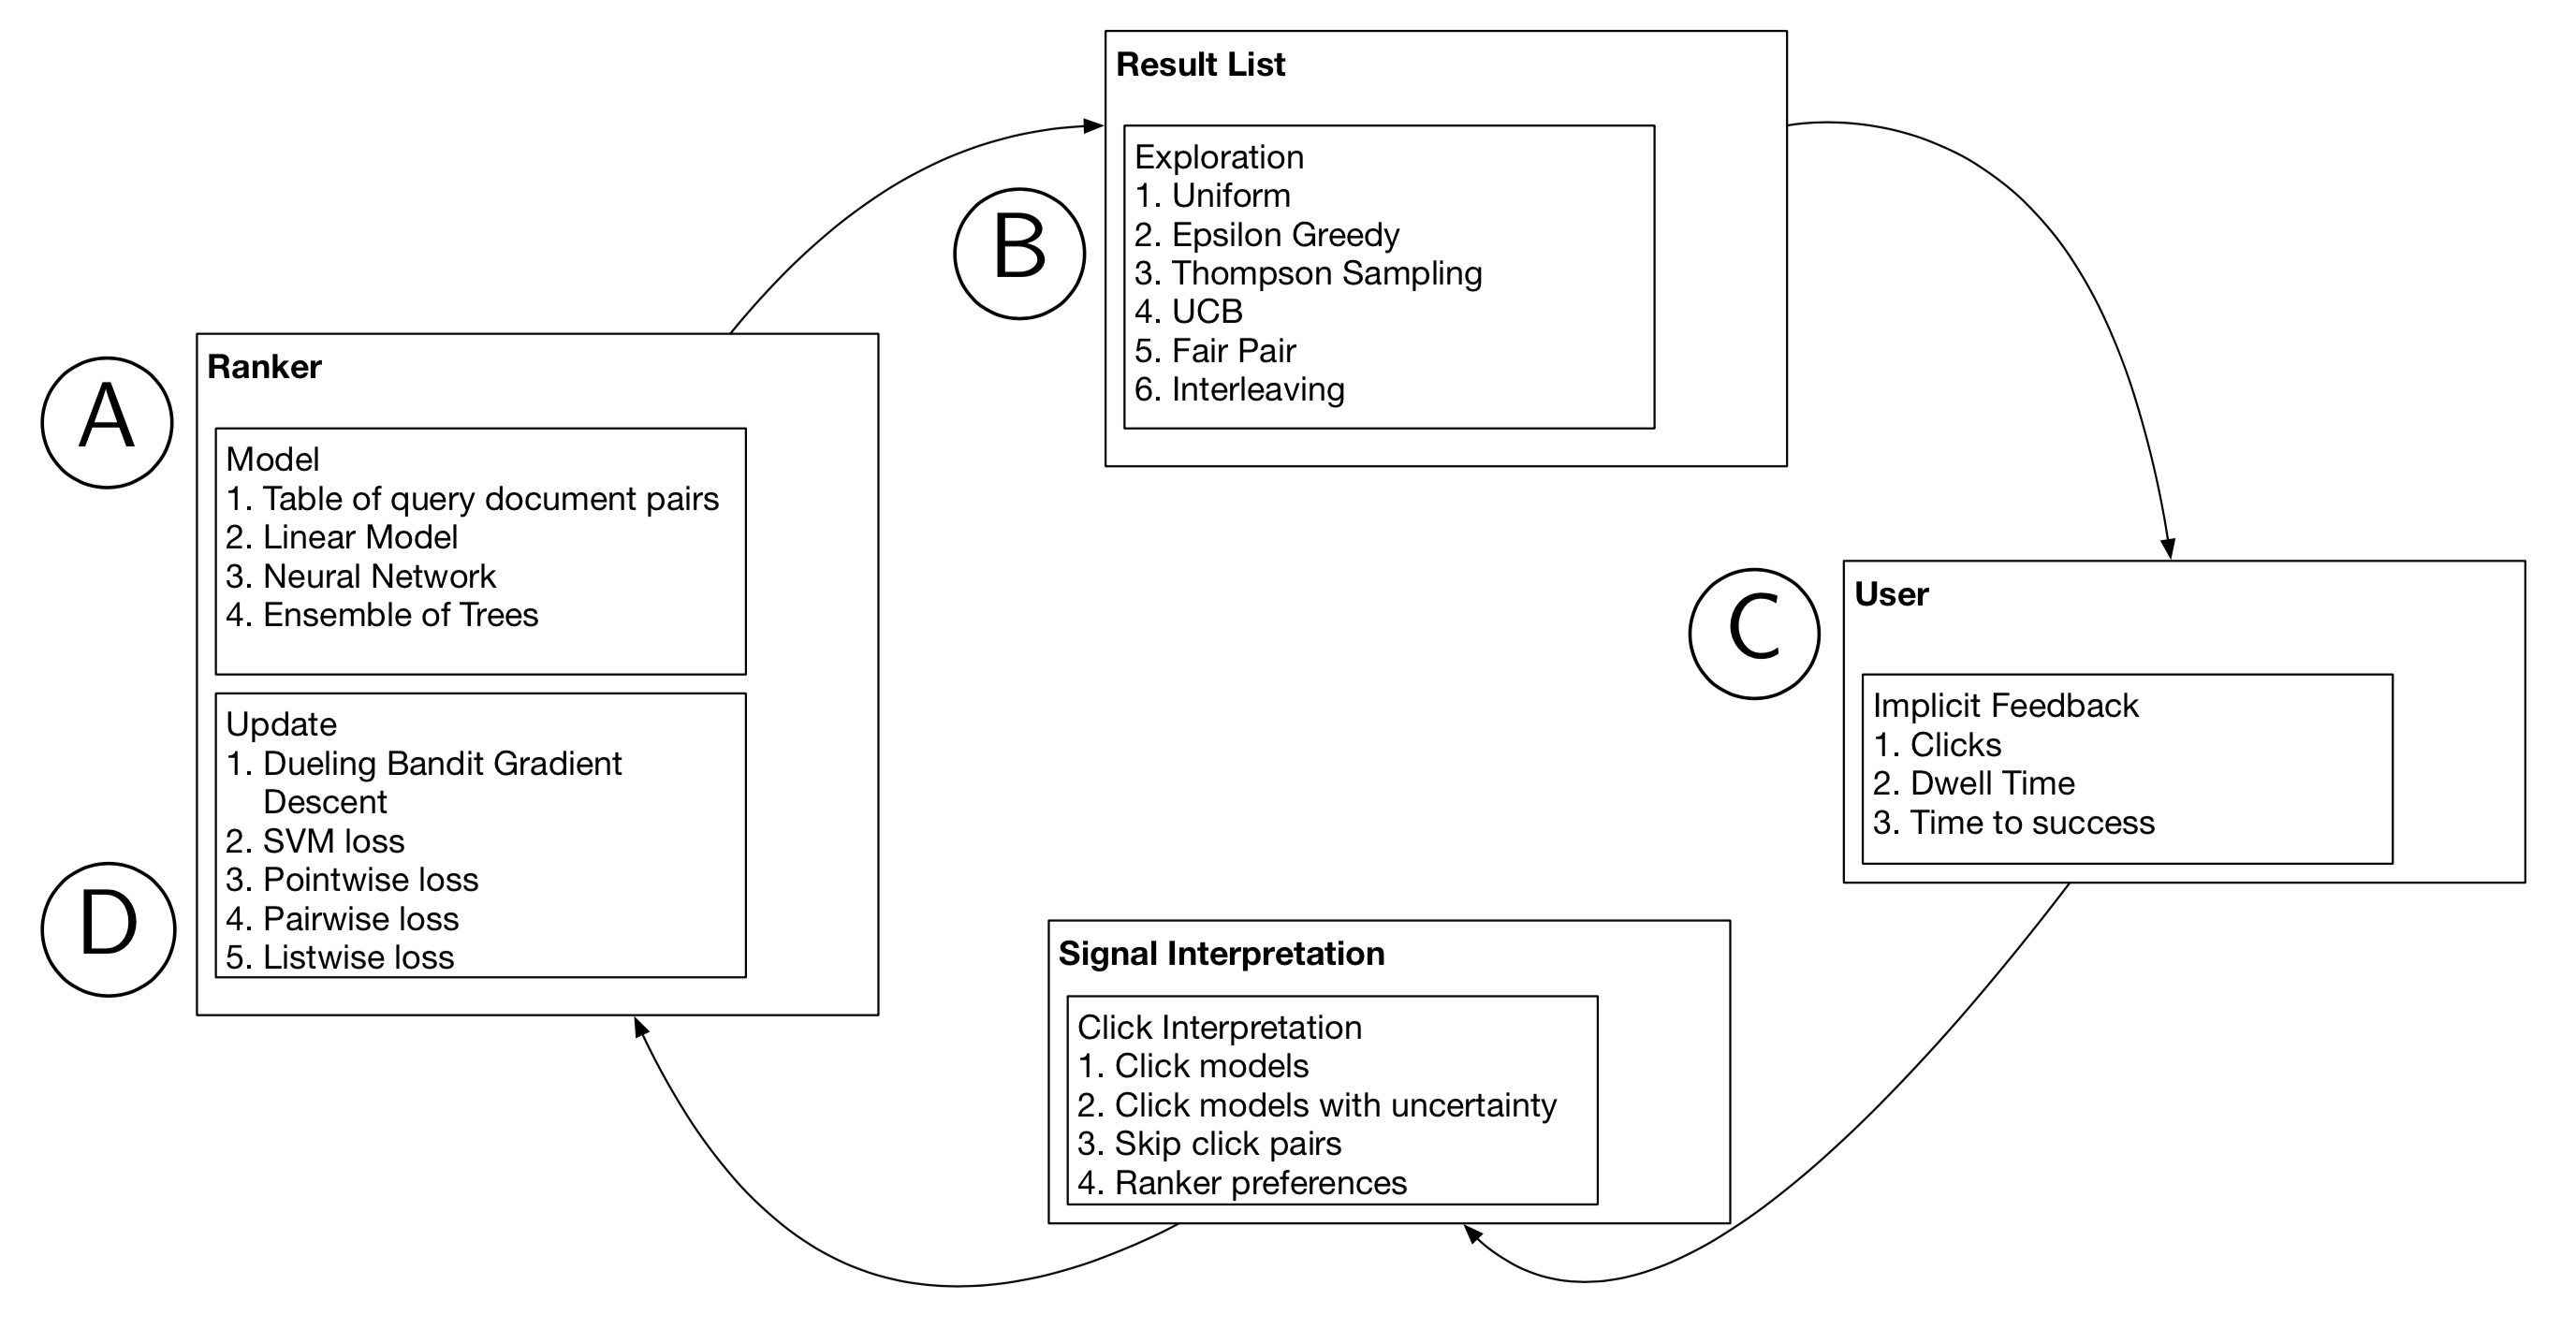
\includegraphics[width=0.4\textwidth]{figures/learning_to_rank_online_design.png}
	\caption{General design components of an OLTR algorithm}
	\label{img:learning_to_rank_online_design}
\end{figure}
\begin{enumerate}[label=(\Alph*)]
	\item \textbf{Ranker}: the ranker maps documents to relevance scores. This module operates on feature level/document id's and can be for example a linear ranker/neural model/...
	\item \textbf{Exploration strategy}: define interactions with results of the ranker. No exploration would mean that the document ranking is simply passed and stays unchanged. A common strategy is \textit{epsilon-greedy} where we inject random documents in random positions with ratio $\epsilon$. Other algorithms include upper confidence bound etc.
	\item \textbf{Signal recording and interpretation}: algorithm can consider multiple signals (raw observation like clicks and dwell time, more complex metrics like time to success). Should remove bias/noise. When result list was constructed by using interleaving, the feedback would also consider which ranker has won based on user interactions.
	\item \textbf{Update mechanism}: update ranking algorithm given the user feedback. If ranker operates on document id's, we can update the document's specific relevance estimate for the query. If the ranker relies on features, we optimize a loss function like the ones shown in offline LTR.
\end{enumerate}
\subsubsection{Dueling Bandit Gradient Descent}
\begin{itemize}
	\item One of the first OLTR algorithms was the \textit{Dueling Bandit Gradient Descent}
	\item The intuition is that we compare two rankers by online evaluation, and optimize our system towards the better performing one.
	\item The method is structured in following steps (visualized in Figure~\ref{img:learning_to_rank_online_DBGD})
	\begin{enumerate}
		\item From current feature state $\theta_b$ of the ranker (shown in green), sample a new ranker/feature point $\theta_c = \theta_b + u$ laying on the unit sphere $||u||=1$ around the current one (shown in red)
		\item Get the rankings of $\theta_b$ and $\theta_c$
		\item Compare $\theta_b$ and $\theta_c$ using interleaving
		\item If $\theta_c$ wins comparison: update the current model by $\theta_b \leftarrow \theta_b + \eta (\theta_c - \theta_b)$
	\end{enumerate}
	\begin{figure}[ht]
		\centering
		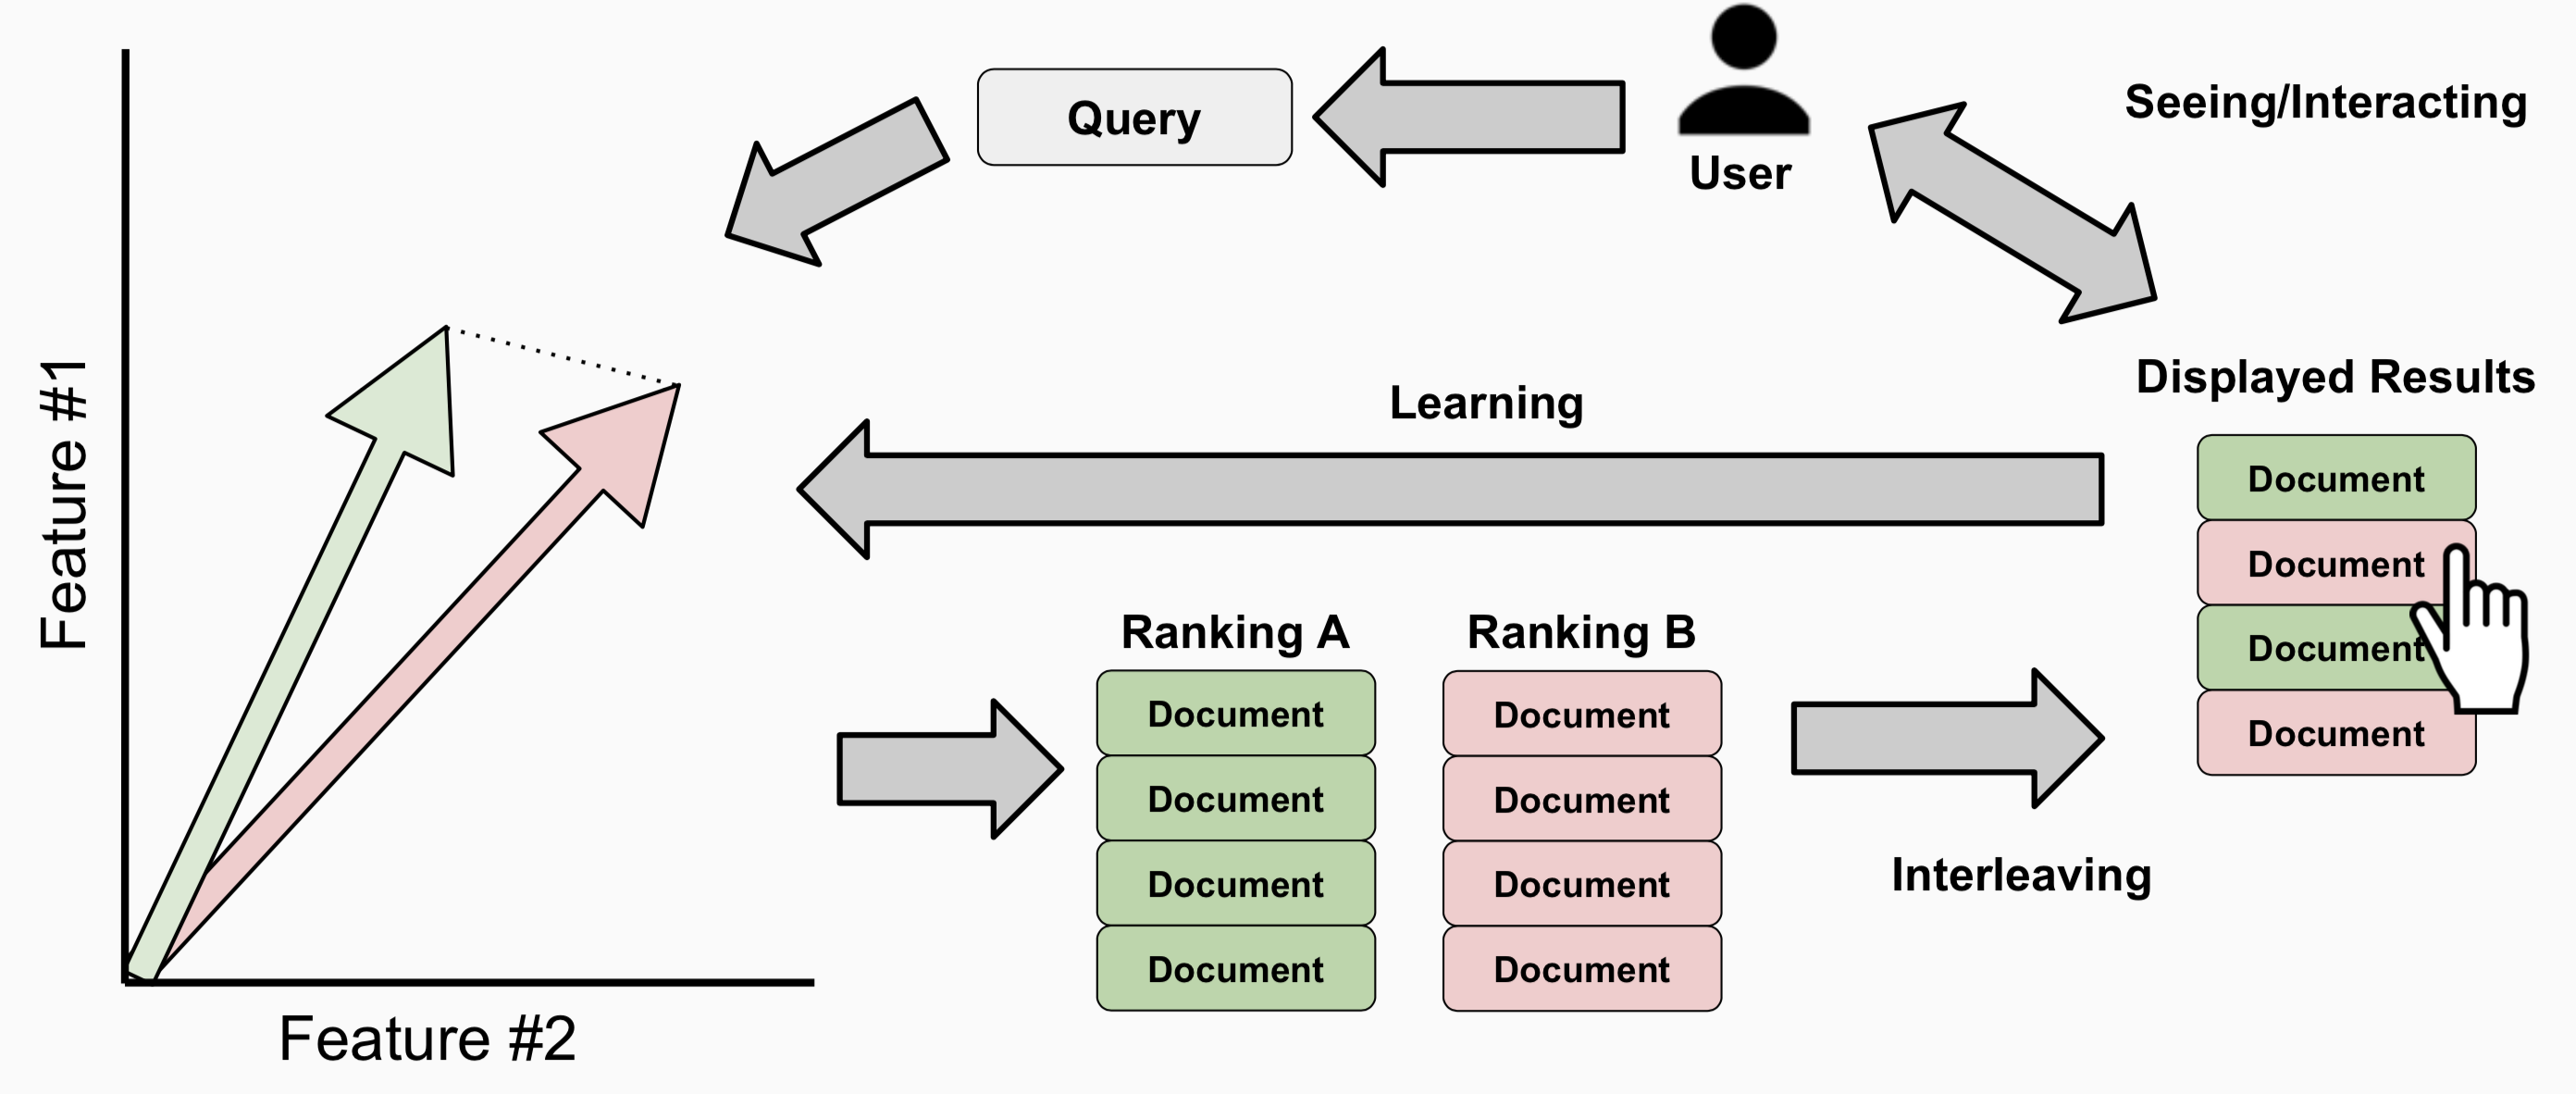
\includegraphics[width=0.5\textwidth]{figures/learning_to_rank_online_DBGD.png}
		\caption{Steps in Dueling Bandit Gradient Descent}
		\label{img:learning_to_rank_online_DBGD}
	\end{figure}
	\item It can be shown that if there is only a single optimum, the Dueling Bandit Gradient Descent algorithm will be able to approximate the optimal model
\end{itemize}